\documentclass[a4paper,11pt]{article}\usepackage[]{graphicx}\usepackage[]{color}
%% maxwidth is the original width if it is less than linewidth
%% otherwise use linewidth (to make sure the graphics do not exceed the margin)
\makeatletter
\def\maxwidth{ %
  \ifdim\Gin@nat@width>\linewidth
    \linewidth
  \else
    \Gin@nat@width
  \fi
}
\makeatother

\definecolor{fgcolor}{rgb}{0.345, 0.345, 0.345}
\newcommand{\hlnum}[1]{\textcolor[rgb]{0.686,0.059,0.569}{#1}}%
\newcommand{\hlstr}[1]{\textcolor[rgb]{0.192,0.494,0.8}{#1}}%
\newcommand{\hlcom}[1]{\textcolor[rgb]{0.678,0.584,0.686}{\textit{#1}}}%
\newcommand{\hlopt}[1]{\textcolor[rgb]{0,0,0}{#1}}%
\newcommand{\hlstd}[1]{\textcolor[rgb]{0.345,0.345,0.345}{#1}}%
\newcommand{\hlkwa}[1]{\textcolor[rgb]{0.161,0.373,0.58}{\textbf{#1}}}%
\newcommand{\hlkwb}[1]{\textcolor[rgb]{0.69,0.353,0.396}{#1}}%
\newcommand{\hlkwc}[1]{\textcolor[rgb]{0.333,0.667,0.333}{#1}}%
\newcommand{\hlkwd}[1]{\textcolor[rgb]{0.737,0.353,0.396}{\textbf{#1}}}%
\let\hlipl\hlkwb

\usepackage{framed}
\makeatletter
\newenvironment{kframe}{%
 \def\at@end@of@kframe{}%
 \ifinner\ifhmode%
  \def\at@end@of@kframe{\end{minipage}}%
  \begin{minipage}{\columnwidth}%
 \fi\fi%
 \def\FrameCommand##1{\hskip\@totalleftmargin \hskip-\fboxsep
 \colorbox{shadecolor}{##1}\hskip-\fboxsep
     % There is no \\@totalrightmargin, so:
     \hskip-\linewidth \hskip-\@totalleftmargin \hskip\columnwidth}%
 \MakeFramed {\advance\hsize-\width
   \@totalleftmargin\z@ \linewidth\hsize
   \@setminipage}}%
 {\par\unskip\endMakeFramed%
 \at@end@of@kframe}
\makeatother

\definecolor{shadecolor}{rgb}{.97, .97, .97}
\definecolor{messagecolor}{rgb}{0, 0, 0}
\definecolor{warningcolor}{rgb}{1, 0, 1}
\definecolor{errorcolor}{rgb}{1, 0, 0}
\newenvironment{knitrout}{}{} % an empty environment to be redefined in TeX

\usepackage{alltt}
\usepackage[utf8]{inputenc}
\usepackage[T1]{fontenc}
\usepackage{graphicx}
\usepackage{amsmath}
%\usepackage{mathtools}
\usepackage[margin=1in]{geometry}
\usepackage{setspace}
  \onehalfspacing
\usepackage{hyperref}
\hypersetup{colorlinks,citecolor=black,filecolor=black,linkcolor=black,urlcolor=black}
\usepackage{tabularx}
\usepackage[round]{natbib}

\title{A Study on the Volatility of Stock Returns of Intel Corporation}
\author{Zheng Tian \\
        Zheng Tian}
\IfFileExists{upquote.sty}{\usepackage{upquote}}{}
\begin{document}

\maketitle
\section{Introduction}
\label{sec:intro}

This document is to show an application of modeling volatility of stock returns using ARCH and GARCH models. The detailed explanation is in Chapter 4 in \citet{Tsay2013}. 





\section{Data Description}
\label{sec:data_descrip}

\subsection*{Basic description}

The data source that we consider is the monthly log stock returns of Intel Corporation from January 1973 to December 2009 for 444 observations. Table \ref{tab:descp_stats} shows the descriptive statistics, and Figure \ref{fig:plot-lnrtn} displays the time plot of the returns. 



% latex table generated in R 3.3.2 by xtable 1.8-2 package
% Tue May 16 16:51:00 2017
\begin{table}[ht]
\centering
\caption{The descriptive statistics of the monthly
                  log stock returns of Intel Corp.} 
\label{tab:descp_stats}
\begin{tabular}{rrrrrrrrr}
  \hline
 & nobs & Minimum & Maximum & 1. Quartile & 3. Quartile & Stdev & Skewness & Kurtosis \\ 
  \hline
1 & 444.00 & -0.60 & 0.49 & -0.05 & 0.10 & 0.13 & -0.55 & 3.12 \\ 
   \hline
\end{tabular}
\end{table}


\begin{knitrout}
\definecolor{shadecolor}{rgb}{0.969, 0.969, 0.969}\color{fgcolor}\begin{figure}

{\centering 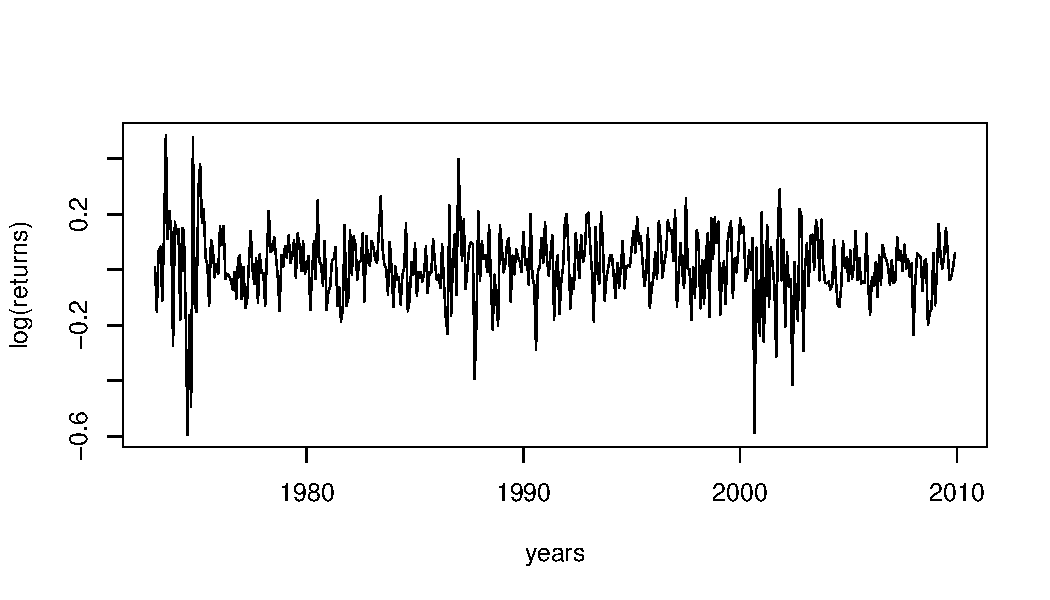
\includegraphics[width=\maxwidth]{figure/plot-lnrtn-1} 

}

\caption[Time plot of the monthly log returns of Intel stock]{Time plot of the monthly log returns of Intel stock}\label{fig:plot-lnrtn}
\end{figure}


\end{knitrout}

\subsection*{Checking stationarity of the Intel stock returns series}



Figure \ref{fig:plot-acf} shows that sample ACF of the log returns and the absolute log returns. There is no significant serial correlations in the log returns except for some minor ones at lags 7 and 14. The Ljung-Box statistic for $\log(r_t)$ shows that $Q(12)$ = 18.68, and the p-value is 0.0967, confirming that there is no serial correlation at the first 12 lags. On the other hand, the Ljung-Box statistic for $|\log(r_t)|$ shows that $Q(12)$ = 124.91 with the p-value being 0, rejecting the null hypothesis of no serial correlation. Consequently, the monthly log returns of Intel stock are serially correlated but dependent. 

\begin{knitrout}
\definecolor{shadecolor}{rgb}{0.969, 0.969, 0.969}\color{fgcolor}\begin{figure}

{\centering 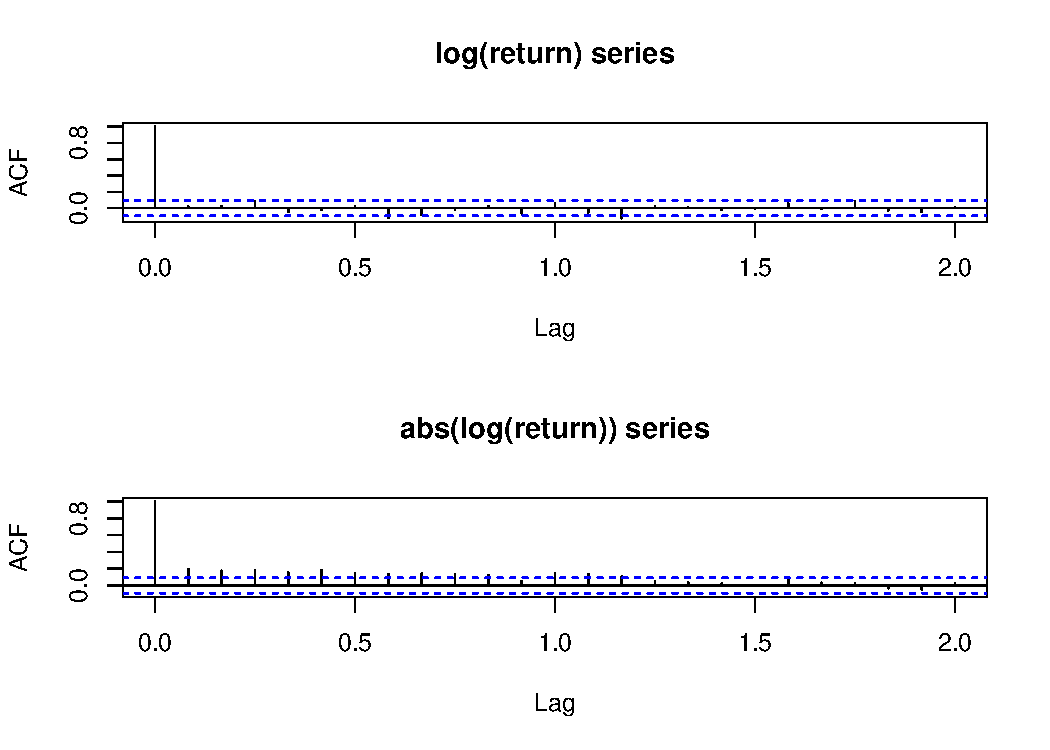
\includegraphics[width=\maxwidth]{figure/plot-acf-1} 

}

\caption[Sample ACF of the monthly log returns of Intel stock]{Sample ACF of the monthly log returns of Intel stock}\label{fig:plot-acf}
\end{figure}


\end{knitrout}

\subsection*{Detecting ARCH effect}



We can use the Ljung-Box test for {$a^2_t$} to test whether there is an ARCH effect in the innovation series calculated from the log return series. The Ljung-Box statistic, $Q(12)$, is 92.94 with the p-value being 0, rejecting the null hypothesis and confirming the ARCH effects. 

\section{The Volatility Model}
\label{sec:volatility_model}

\subsection*{The ARCH model}

We first build an ARCH(3) model with the Gaussian $\epsilon_t$ and then estimate an ARCH(1) model because only $\alpha_1$ is significant in the ARCH(3) model. Then, we replace the normal distribution with a Student-t distribution. All the results are reported in Table \ref{tab:arch-results}. 

\begin{equation}
r_t = \mu + a_t,\, 
a_t = \sigma_t \epsilon_t,\, 
\epsilon^2_{t}=\alpha_0 + \alpha_1 a^2_{t-1} + \alpha_2 a^2_{t-2} 
+ \alpha_3 a^2_{t-3}
\end{equation}








\begin{table}[!htbp] \centering 
  \caption{The Estimation Results of ARCH Models} 
  \label{tab:arch-results} 
\begin{tabular}{@{\extracolsep{5pt}}lccc} 
\\[-1.8ex]\hline 
\hline \\[-1.8ex] 
 & \multicolumn{3}{c}{\textit{Dependent variable:}} \\ 
\cline{2-4} 
\\[-1.8ex] & (1) & (2) & (3)\\ 
\hline \\[-1.8ex] 
 mu & 0.013$^{**}$ & 0.013$^{**}$ & 0.017$^{***}$ \\ 
  & (0.006) & (0.005) & (0.005) \\ 
  & & & \\ 
 omega & 0.010$^{***}$ & 0.011$^{***}$ & 0.012$^{***}$ \\ 
  & (0.001) & (0.001) & (0.002) \\ 
  & & & \\ 
 alpha1 & 0.233$^{**}$ & 0.375$^{***}$ & 0.277$^{***}$ \\ 
  & (0.112) & (0.113) & (0.107) \\ 
  & & & \\ 
 alpha2 & 0.075 &  &  \\ 
  & (0.047) &  &  \\ 
  & & & \\ 
 alpha3 & 0.052 &  &  \\ 
  & (0.045) &  &  \\ 
  & & & \\ 
 shape &  &  & 5.970$^{***}$ \\ 
  &  &  & (1.530) \\ 
  & & & \\ 
\hline \\[-1.8ex] 
Observations & 444 & 444 & 444 \\ 
Log Likelihood & $-$303.961 & $-$299.925 & $-$315.090 \\ 
Akaike Inf. Crit. & $-$1.347 & $-$1.337 & $-$1.401 \\ 
Bayesian Inf. Crit. & $-$1.301 & $-$1.310 & $-$1.364 \\ 
\hline 
\hline \\[-1.8ex] 
\textit{Note:}  & \multicolumn{3}{r}{$^{*}$p$<$0.1; $^{**}$p$<$0.05; $^{***}$p$<$0.01} \\ 
\end{tabular} 
\end{table} 


The log-likelihood function and AIC point to the ARCH(1) model, while BIC points to the ARCH(3) model. We check the model adequacy by testing autocorrelation in the stardardized residuals and squared residuals. 

\begin{knitrout}
\definecolor{shadecolor}{rgb}{0.969, 0.969, 0.969}\color{fgcolor}
\begin{figure}
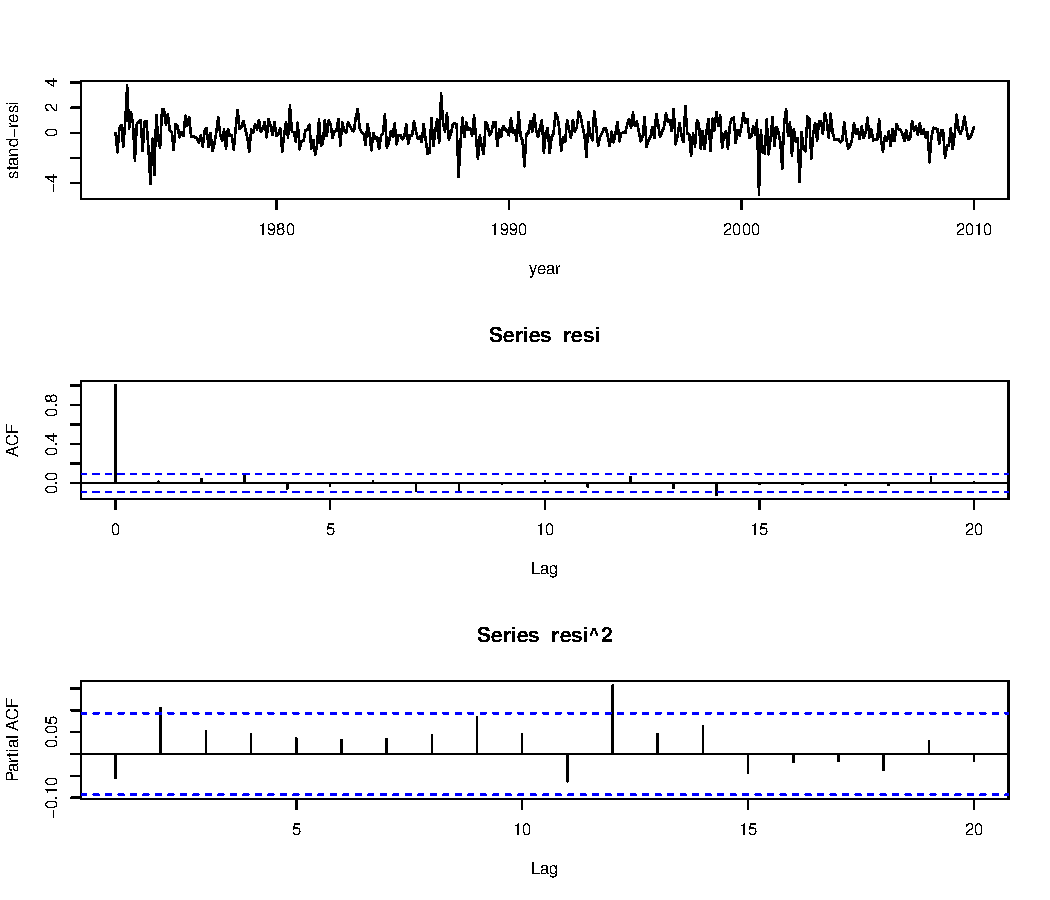
\includegraphics[width=\maxwidth]{figure/model-checking-resid-1} 
\caption[Model checking of the Gaussian ARCH(1) model]{Model checking of the Gaussian ARCH(1) model}\label{fig:model-checking-resid}
\end{figure}


\end{knitrout}

\subsection*{The GARCH model}

While the ARCH models fit the data well, there is still some correlation in the squared standardized residuals at the lags after 10. Instead of adding many lagged terms in an ARCH model, we entertain a GARCH(1, 1,) model for the log return series for the sake of parsimony. 

A GARCH(1, 1) model is as follows
\begin{align*}
r_t &= \mu + a_t,\, a_t = \sigma_t \epsilon_t,\, \epsilon_t \sim N(0, 1) \\
\sigma^2_t &= \alpha_0 + \alpha_1 a^2_{t-1} + \beta_1 \sigma^2_{t-1}
\end{align*}

We plot the fitted volatility and the standardized residuals from the GARCH(1, 1) model in Figure \ref{fig:plot-garch}. Next, we check model adequacy the ACF of {$\tilde{a}_t$} and {$\tilde{a}^2_t$} in Figure \ref{fig:model-chk-garch}. And add the predicative intervals to the log return series in Figure \ref{fig:predict-intval}.



\begin{knitrout}
\definecolor{shadecolor}{rgb}{0.969, 0.969, 0.969}\color{fgcolor}\begin{figure}
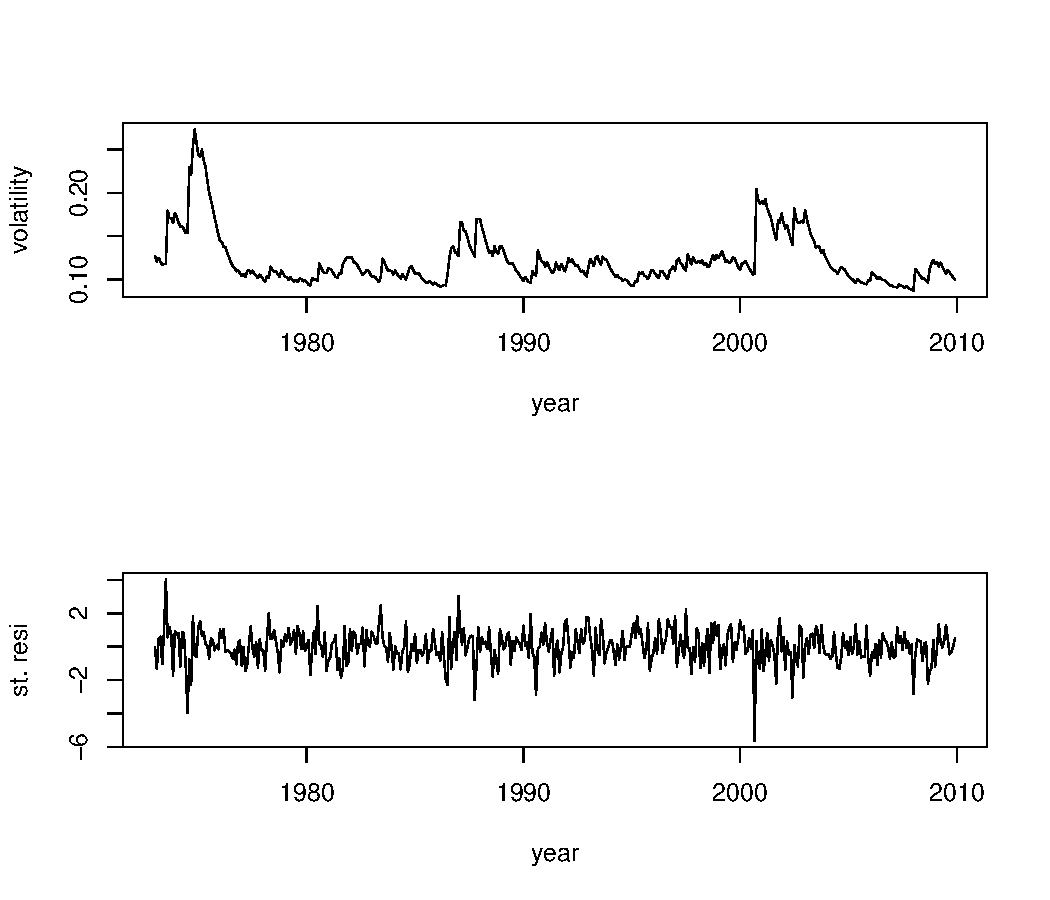
\includegraphics[width=\maxwidth]{figure/plot-garch-1} \caption[Time plots for a fitted Gaussian GARCH(1, 1) model]{Time plots for a fitted Gaussian GARCH(1, 1) model}\label{fig:plot-garch}
\end{figure}


\end{knitrout}

\begin{knitrout}
\definecolor{shadecolor}{rgb}{0.969, 0.969, 0.969}\color{fgcolor}\begin{figure}
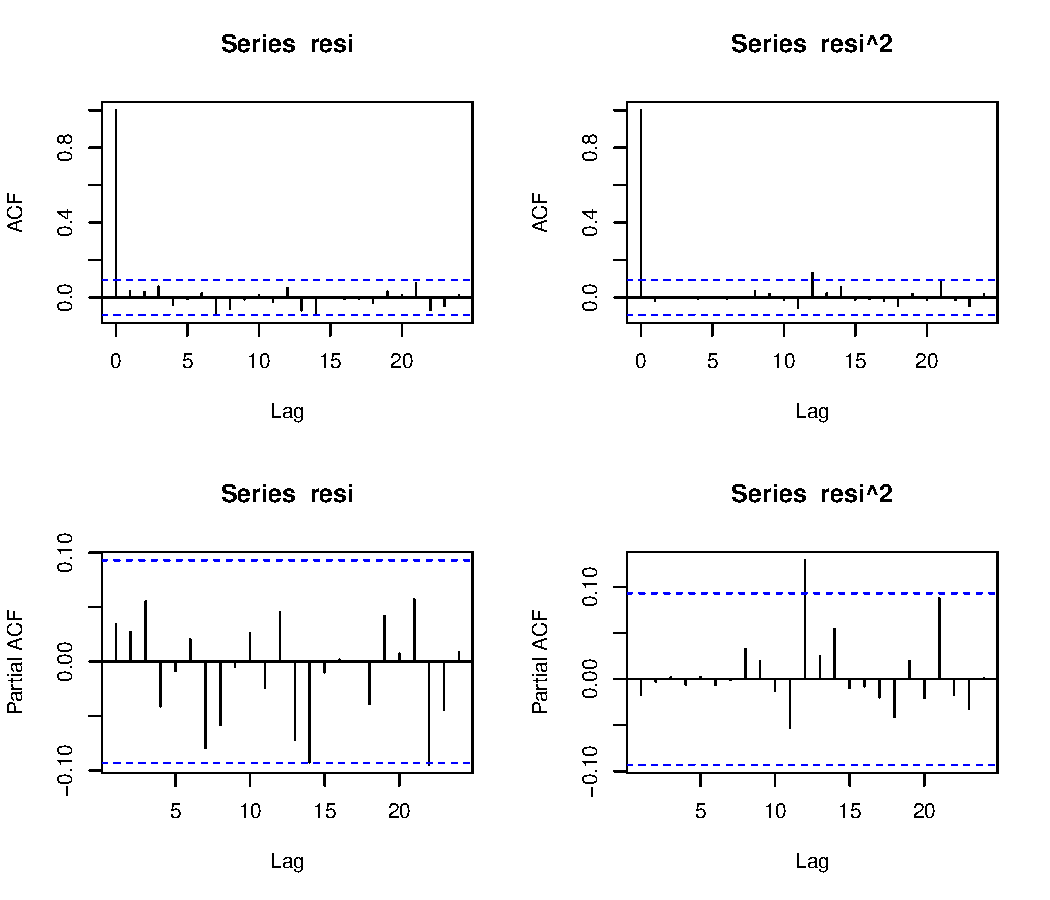
\includegraphics[width=\maxwidth]{figure/model-chk-garch-1} \caption[Sample ACF and PACF of the standardized residuals and their squared series of a Gaussian GARCH(1,1) model]{Sample ACF and PACF of the standardized residuals and their squared series of a Gaussian GARCH(1,1) model}\label{fig:model-chk-garch}
\end{figure}


\end{knitrout}

\begin{knitrout}
\definecolor{shadecolor}{rgb}{0.969, 0.969, 0.969}\color{fgcolor}\begin{figure}
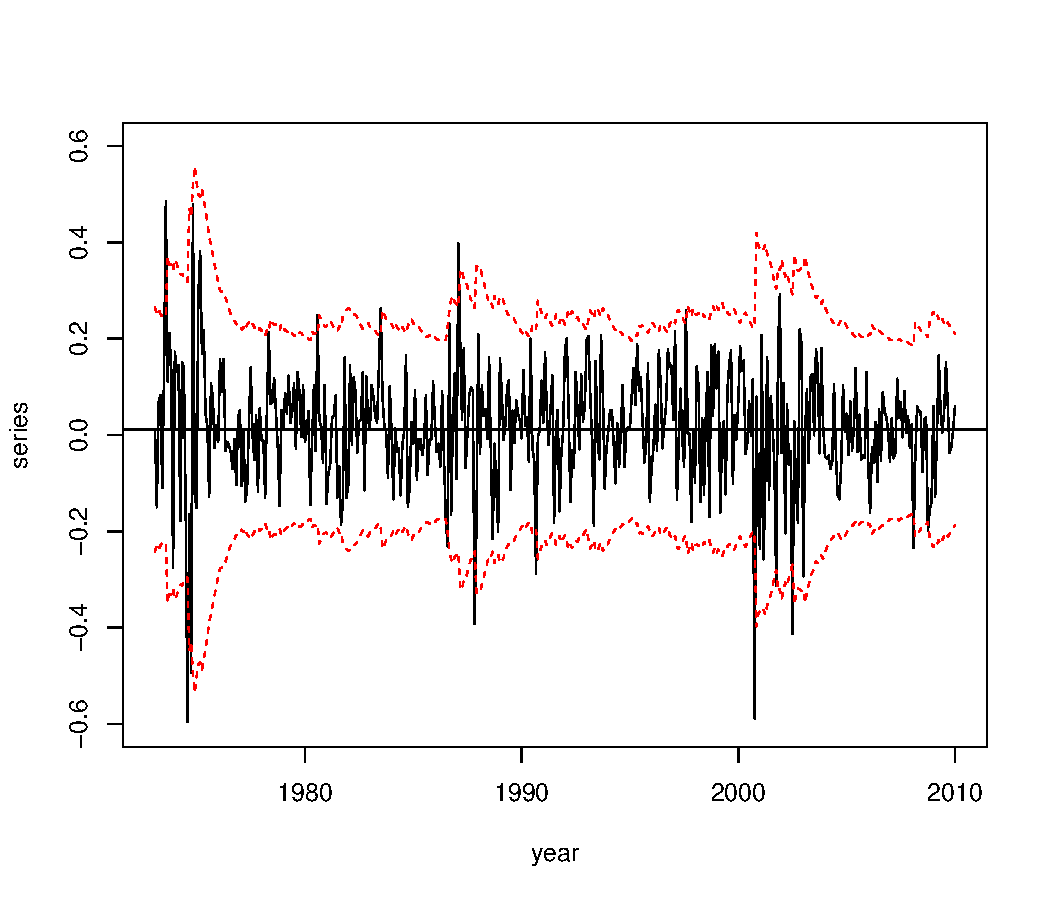
\includegraphics[width=\maxwidth]{figure/predict-intval-1} \caption[Time plot of the monthly log returns of Intel stock with the point-wise predicative intervals]{Time plot of the monthly log returns of Intel stock with the point-wise predicative intervals}\label{fig:predict-intval}
\end{figure}


\end{knitrout}

\section{Conclusion}
\label{sec:conclusion}

\bibliography{fda}
\bibliographystyle{unsrtnat}


\end{document}
